\documentclass[preprint,12pt]{elsarticle}
\usepackage{amsmath}
\usepackage[utf8]{inputenc}

%% Use the option review to obtain double line spacing
%% \documentclass[preprint,review,12pt]{elsarticle}

%% Use the options 1p,twocolumn; 3p; 3p,twocolumn; 5p; or 5p,twocolumn
%% for a journal layout:
%% \documentclass[final,1p,times]{elsarticle}
%% \documentclass[final,1p,times,twocolumn]{elsarticle}
%% \documentclass[final,3p,times]{elsarticle}
%% \documentclass[final,3p,times,twocolumn]{elsarticle}
%% \documentclass[final,5p,times]{elsarticle}
%% \documentclass[final,5p,times,twocolumn]{elsarticle}

%% The graphicx package provides the includegraphics command.
\usepackage{graphicx}
%% The amssymb package provides various useful mathematical symbols
\usepackage{amssymb}
%% The amsthm package provides extended theorem environments
%% \usepackage{amsthm}
%% The lineno packages adds line numbers. Start line numbering with
%% \begin{linenumbers}, end it with \end{linenumbers}. Or switch it on
%% for the whole article with \linenumbers after \end{frontmatter}.
\usepackage{lineno}
%% natbib.sty is loaded by default. However, natbib options can be
%% provided with \biboptions{...} command. Following options are
%% valid:

\journal{Biological Physics 275, UCSD}

\begin{document}

\begin{frontmatter}

%% Title, authors and addresses

\title{A two-state system of diffusion models dimorphic fungal morphogenesis and mycelial growth}

%% use the tnoteref command within \title for footnotes;
%% use the tnotetext command for the associated footnote;
%% use the fnref command within \author or \address for footnotes;
%% use the fntext command for the associated footnote;
%% use the corref command within \author for corresponding author footnotes;
%% use the cortext command for the associated footnote;
%% use the ead command for the email address,
%% and the form \ead[url] for the home page:
%%
%% \title{Title\tnoteref{label1}}
%% \tnotetext[label1]{}
%% \author{Name\corref{cor1}\fnref{label2}}
%% \ead{email address}
%% \ead[url]{home page}
%% \fntext[label2]{}
%% \cortext[cor1]{}
%% \address{Address\fnref{label3}}
%% \fntext[label3]{}


%% use optional labels to link authors explicitly to addresses:
%% \author[label1,label2]{<author name>}
%% \address[label1]{<address>}
%% \address[label2]{<address>}

\author{Cameron Martino}

\address{University of California San Diego, La Jolla, CA, USA}

\begin{abstract}
%% Text of abstract
Dimorphic fungi transition from filamentous to yeast-like morphologies in the infection of host tissues or blood. In dimorphic fungi, morphogenesis is induced through temperature transitions, where both morphologies often grow in mycelial like biofilm. The treatment of dimorphic fungal infections relies heavily on the use of fungicides. However, due to native resistances, dimorphic fungal infections can require fungicide concentrations that cause negative impacts on the host. This is further complicated by the time-consuming process of testing fungicide susceptibility through low minimum inhibitory concentrations (MIC) which do not fully replicate host conditions. Therefore, having a simple model of morphological proportions over temperature and how biofilm spreads radially could give insight into this unique niche of microorganisms. Here, a two-state system is proposed to be a good model of dimorphic fungal morphogenesis. Additionally, Fick’s law of diffusion and the Stokes–Einstein equation are proposed to be good analytical models of radial mycelial growth. \\
\end{abstract}

\end{frontmatter}
\linenumbers

%% main text
The Fungal kingdom, comprised of yeasts and molds, are known to be integral in environmental and host-associated microbial ecology. Of primary importance in medical mycology are pathogenic fungi with dimorphic lifestyles. Dimorphic fungi can alternate between a mold and yeast-like state, in some cases, capable of forming pseudohyphal networks \cite{Veses2009-ly}. The mold state is more often found in the environment growing in multicellular filaments called hyphae. While, when found in a host-associated environment they exist more often in a single cell -- budding yeast-like state. This morphological change is characterized by temperature change where the cold is associated with the mold like state. A popular mnemonic is “Mold in the Cold, Yeast in the Heat”, which is true for all but a few dimorphic fungi. Here, as a case study, we will primarily focus on a model pathogenic dimorphic fungus, \textit{Blastomyces dermatitidis} (Onygenales, Ascomycota), the cause of blastomycosis, an atopic skin disease endemic to North America. However, the models proposed here are globally applicable to most dimorphic fungi. \\ \par

\textit{Blastomyces dermatitidis} is known to transition from mold state to yeast state at a temperature change between 25 to 37 $C^{o.}$ The first molecular characterization of the dimorphic switch described a three-step cascade \citep{Medoff1987-kt}. Characterized by an uncoupling of oxidative phosphorylation and a decrease in ATP, respiration and electron transport (step 1). Then spontaneous respiration ceases in the presence of cysteine (step 2) and finally a recovery into yeast state (step 3).  Step 1 has been further characterized genomically as a two-component signaling system called Hybrid Histidine Kinase (HHK) and was found to be globally regulating for all known pathogenic dimorphic fungi \citep{Nemecek2006-ff}. This signaling system functions through four sequential phosphorylation events. First, HHK is stimulated from external stimuli and is autophosphorylated. The phosphate is then transferred to an aspartate in the HHK cytoplasmic response regulator (RR) domain. Second, the phosphate group is moved to a phosphotransfer protein (HPt) where it is then transferred to a second RR domain. This process is differentiated into 11 classes of HHK across different fungi based on the complexity of lifecycle.  However, in all known dimorphic species, there are still only two RR events giving four phosphorylation events \citep{Catlett2003-mn}. Knockouts of these genes also result in the prevention of dimorphic progression and pathogenesis \citep{Nemecek2006-ff}. \\ \par

Additionally, the use of miRNA to silence expression of the cascade proved an effective tool against dimorphic fungal infection in mice \citep{Nemecek2006-ff}.  However, currently, fungal infections are treated with fungicide. This practice can be complicated by the native resistance to most known fungicides by dimorphic fungi \citep{Goughenour2017-xk}. This causes the use of fungicide concentrations that can be detrimental to host health in order to prevent the spread of infection. Further complicating this problem is the time taken to perform MIC testing on a clinical isolate for the sensitivity of a given fungicide. Cultivation methods, in this case, may also be complicated in clinical relevance by their similarity or dissimilarity to the host infection conditions (i.e. temperature and substrate availability). All of these complications, the known molecular mechanisms for growth, and simple analytical models of physics can provide a framework for a model of both that may be of some biological or clinical relevance. \\ \par


\textbf{\textit{State Modeling of Dimorphic Morphogenesis}}
\newline

There are multiple steps in the phosphorylation cascade that result in morphogenesis. However, the separation of time scales between the time of phosphorylation down the cascade and the change in morphology allows it to be modeled as one event. Therefore, a state variable is given for all phosphorylation events as being globally unphosphorylated ($\sigma_{p}=0$) or phosphorylated ($\sigma_{p}=1$). In this case, the occurrence of phosphorylation is equivalent to the yeast like state and likewise unphosphorylated to the mold like state. \\ \par

Additionally, to control the free energy landscape by temperature, another state variable is introduced for the stable temperature at the cold mold state ($\sigma_{t}=0$) and warmer yeast-like state ($\sigma_{t}=1$). To create a free energy landscape for any paradigm, since not all species convert at the same temperature, $\epsilon_{m}$ is introduced.  Where $\epsilon_{m}$ can be derived empirically from the known temperature preferences by

\begin{equation}
\epsilon_{m} = T_{state} - T_{transition}
\end{equation}
%
where  $T_{state}$ is the optimal temperature for that given morphological state and $T_{transition}$ is the midpoint temperature between the two states (Fig. 1A). This energy landscape can then be solved as the probabilities of a morphological state by temperature as

\begin{equation}
P_{mold} = \frac{1}{1+e^{\epsilon_m}}
\qquad
P_{yeast-like} = \frac{e^{\epsilon_m}}{1+e^{\epsilon_m}}
\qquad
P_{intermediate} = \frac{2e^{\epsilon_m}}{(1+e^{\epsilon_m})^{2}}
\end{equation}
%
where $P_{mold}$, $P_{yeast-like}$ and $P_{intermediate}$ correspond to the probability of mold, yeast-like and an intermediate state for any given $\epsilon_{m}$. When applied to experimental data for cultivation temperatures ranging between 28 to 48 $C^{o}$ from data of \textit{Rhizopus oryzae} in Karmakar et al. \citep{Karmakar2012-le} a good fit to the experimental data is observed with $R^{2}$ values of .99, .99, and .98 for the mold, yeast-like, and intermediate morphologies respectively (Fig. 1B). Although only one case-study was available to demonstrate the validity of the model it provides a convenient model of the proportional morphology found at a given temperature. Furthermore, the experiment to validate the model in other spcies should be relatively simple. For the rest of the models, the temperatures were shifted to represent optimal transitions for \textit{Blastomyces dermatitidis}. \newline

\textbf{\textit{Modeling of Hyphal and Pseudohyphal Growths}}
\newline

Once a dimorphic fungal spore lands in a nutrient-rich environment it will germinate and begin to grow. Often, the global morphology that characterizes the growth after germination is hyphal in cold and pseudohyphal/budding-yeast in warm temperatures. In whole the resulting networks are referred to as mycelium when grown in a biofilm. It has also been observed that at the optimal temperature each morphology will grow to a similar density freely and a similar radius \citep{Nemecek2006-ff}. Therefore, for this model, the states are modeled the same to simplify the problem \citep{Klein2007-ge}. \\

Mycelial network models have been extensively studied in the literature. Here, the simplest model was considered, a 2-dimensional Brownian branching random walk model \citep{Fisher1937-lz} which has been used in the past for mycelial network modeling \citep{Carver2008-bq}. Additionally, substrate use over each branch tip growth was incorporated by Lejeune et al. \citep{Lejeune1995-it}. The substrate utilization by branch length growth over time is modeled through a slight alteration to the Monod equation of bacterial growth \citep{Monod1949-rl} for filament lengths, given by

\begin{equation}
\mu_{t} = \mu_{initial}\frac{l_t}{l_t + k_t}\frac{S_t}{S_t + k_s}
\label{eqn:1}
\qquad
l_{t} = \sqrt{(x-x_i)^{2}-(y-y_i)^{2}}
\label{eqn:1}
\end{equation} 
%
where $\mu_{t}$ is the step length at a given time t,  $\mu_{initial}$ is the initial branch, $k_{t}$ is the saturation constant, $S_{t}$ is the substrate concentration at time t, $k_{s}$ is the half-velocity constant, $x_{i}$ is the initial starting point in x, $y_{i}$ is the initial starting point in y, and x and y at each step are given by

\begin{equation}
x = \mu_{t} \xi cos(\theta)
\qquad
y = \mu_{t} \xi sin(\theta)
\end{equation}
%
where $\xi$ is the persistence length. The initial number of starting branches is given by the number of simultaneously germinating spores at $t_0$. \\

However, this simulation based solution requires a lot of variables to determine. Therefore, an simpler analytical solution may be more appropriate. To this end Fick's law of diffusion \cite{Fick1855-zf} utilizing the Stokes–Einstein equation \cite{Einstein1956-yu} was used to model root-mean-square deviation (RMSD) given by

\begin{equation}
r_{RMSD} = \sqrt{6Dt}
\qquad
D = \frac{K_{b}T}{f}
\end{equation}
%
where D is the diffusion constant, $k_{b}$ is Boltzmann's constant, and $f$ is the friction factor. \\

Using data on \textit{Blastomyces dermatitidis} from supplemental figure 1 of Nemecek et al. \citep{Nemecek2006-ff} $\mu_{intial}$ was derived empirically to be 75 $\frac{\mu m}{hour}$ with an $S_0$=2350 mg. In Nemecek et al. a culture duration of 60 days produced a mycelial radius of 4 cm giving $D = .04$ and $f = 1.2e^{-20}$. Comparing the analytical ($R^{2}=0.99$) and simulation ($R^{2}=0.91$) the analytical solution proved to be a better fit (Fig. 2). \newline

\textbf{\textit{Characterizing growth radius over temperature}}
\newline

Growth rates in both free growing microbes and mycelial networks have been shown to be dependent on temperature \citep{Domingues2016-jd,Lopez-Moral2017-qi,Moral2011-az}. In order to properly model the growth within the context of the unique temperature induced morphogensis of dimorphic fungi (Fig. 3A) a simple integration of the two-state model from the previous section and the Stokes–Einstein equation \cite{Einstein1956-yu} is given by 

\begin{equation}
\begin{aligned}
D_{mold} = \frac{K_{b}T_{mold}}{f}\frac{1}{1+e^{\epsilon_m}} \\ 
D_{yeast-like} = \frac{K_{b}T_{yeast-like}}{f}\frac{e^{\epsilon_m}}{1+e^{\epsilon_m}} \\
D_{intermediate} = \frac{K_{b}T_{yeast-like}}{f}\frac{2e^{\epsilon_m}}{(1+e^{\epsilon_m})^{2}} \\
\end{aligned}
\end{equation}
\\
This allows for an estimate of the radial growth over time at each temperature. This also predicts a dramatic radial growth drop off for \textit{Blastomyces dermatitidis} below 35 $C^{o}$ (Fig. 3B). No dataset known by the author can be used to benchmark this result. However, this analytical model only relies on very few variables which can be fit for any clinical isolate in the presence of antifungal at a experimental concentration. These results also demonstrate that a simple analytical solution can accurately model complex dimorphic mycelial growth.  \\
 
%% References
\textbf{\textit{Citations}}
\bibliographystyle{model1-num-names}
\bibliography{phys.bib} 

%% Figures 
\pagebreak
\begin{figure}[h]
\centering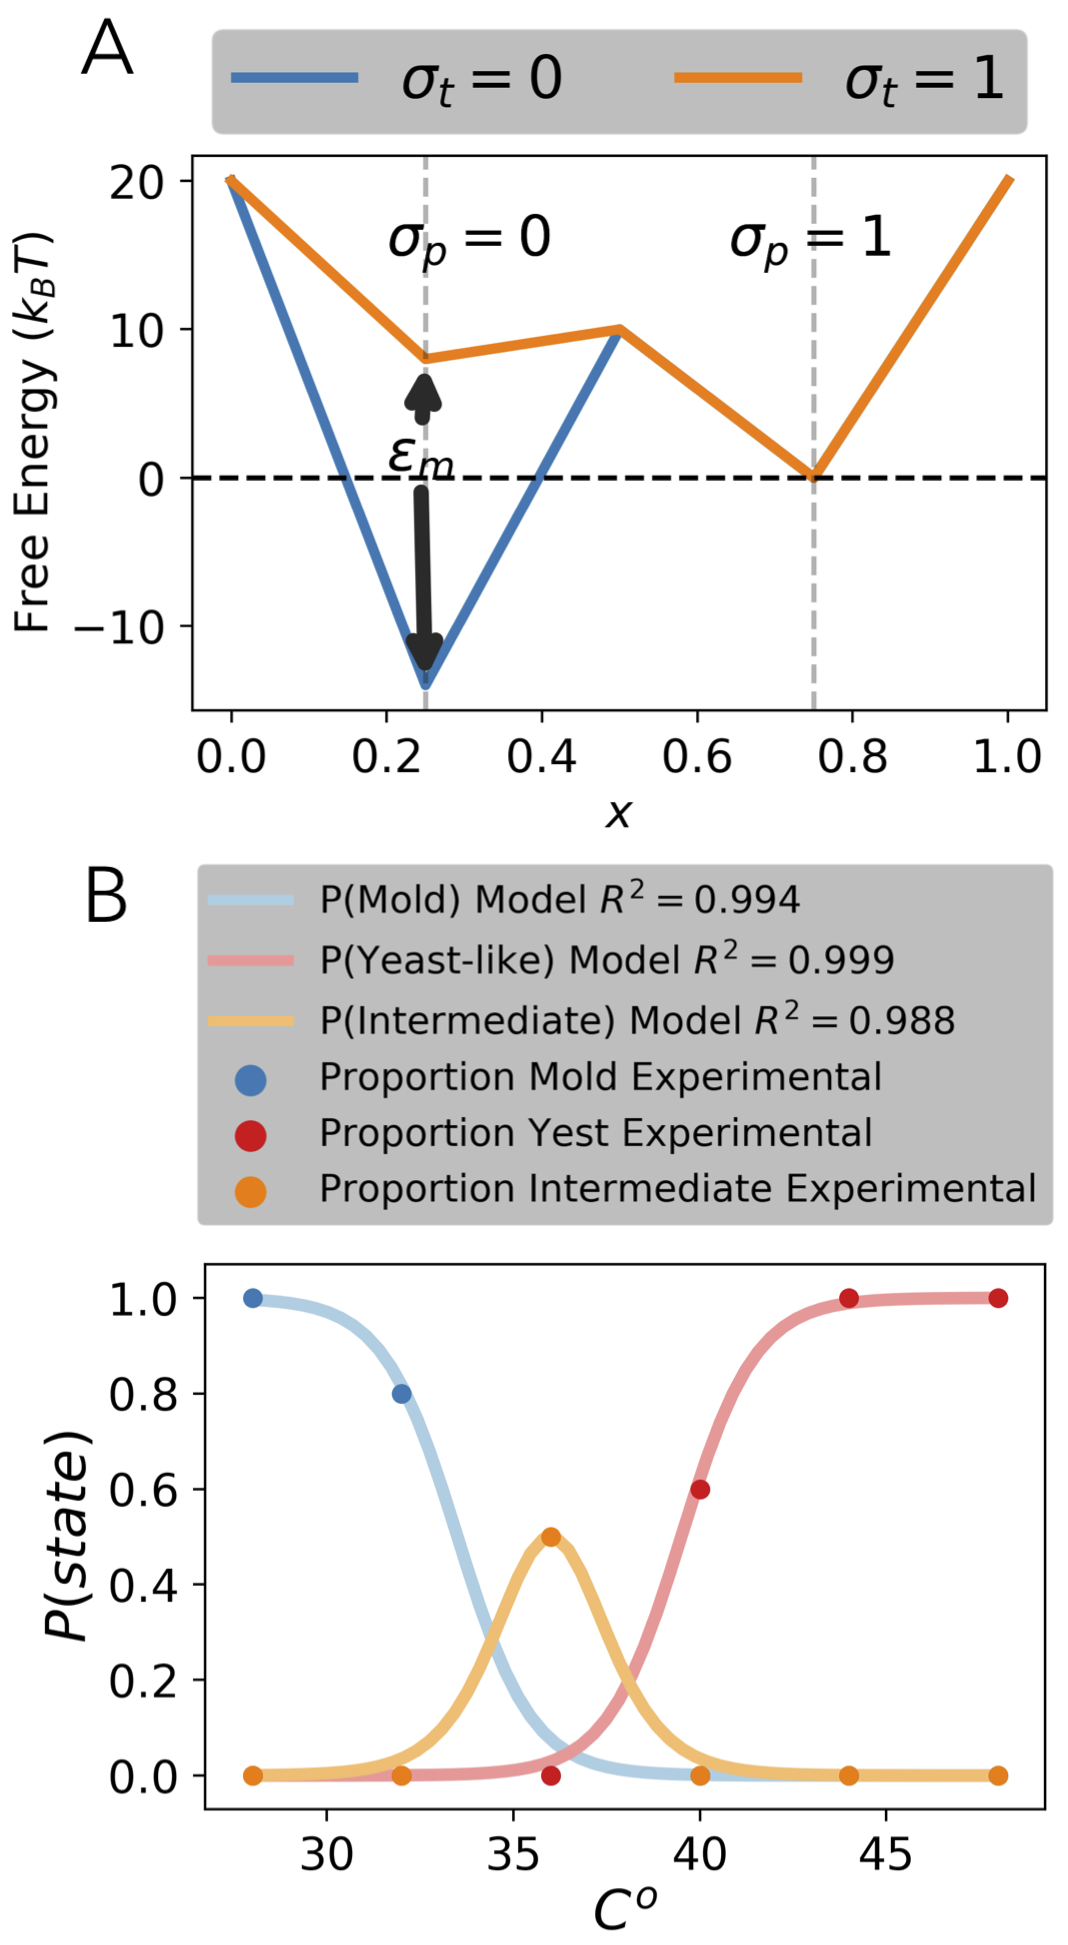
\includegraphics[width=.75\linewidth]{fig1.png}
\caption{Free energy landscape with two state variables $\simga_{t}$ and $\simga_{p}$ plotted by free energy (y-axis) and the distance in the phosphorylation binding (x-axis) (A). Plot comparing the model fit (solid line) to the experimental data (scatter plot) for each morphology state (B).}
\end{figure}

\begin{figure}[h]
\centering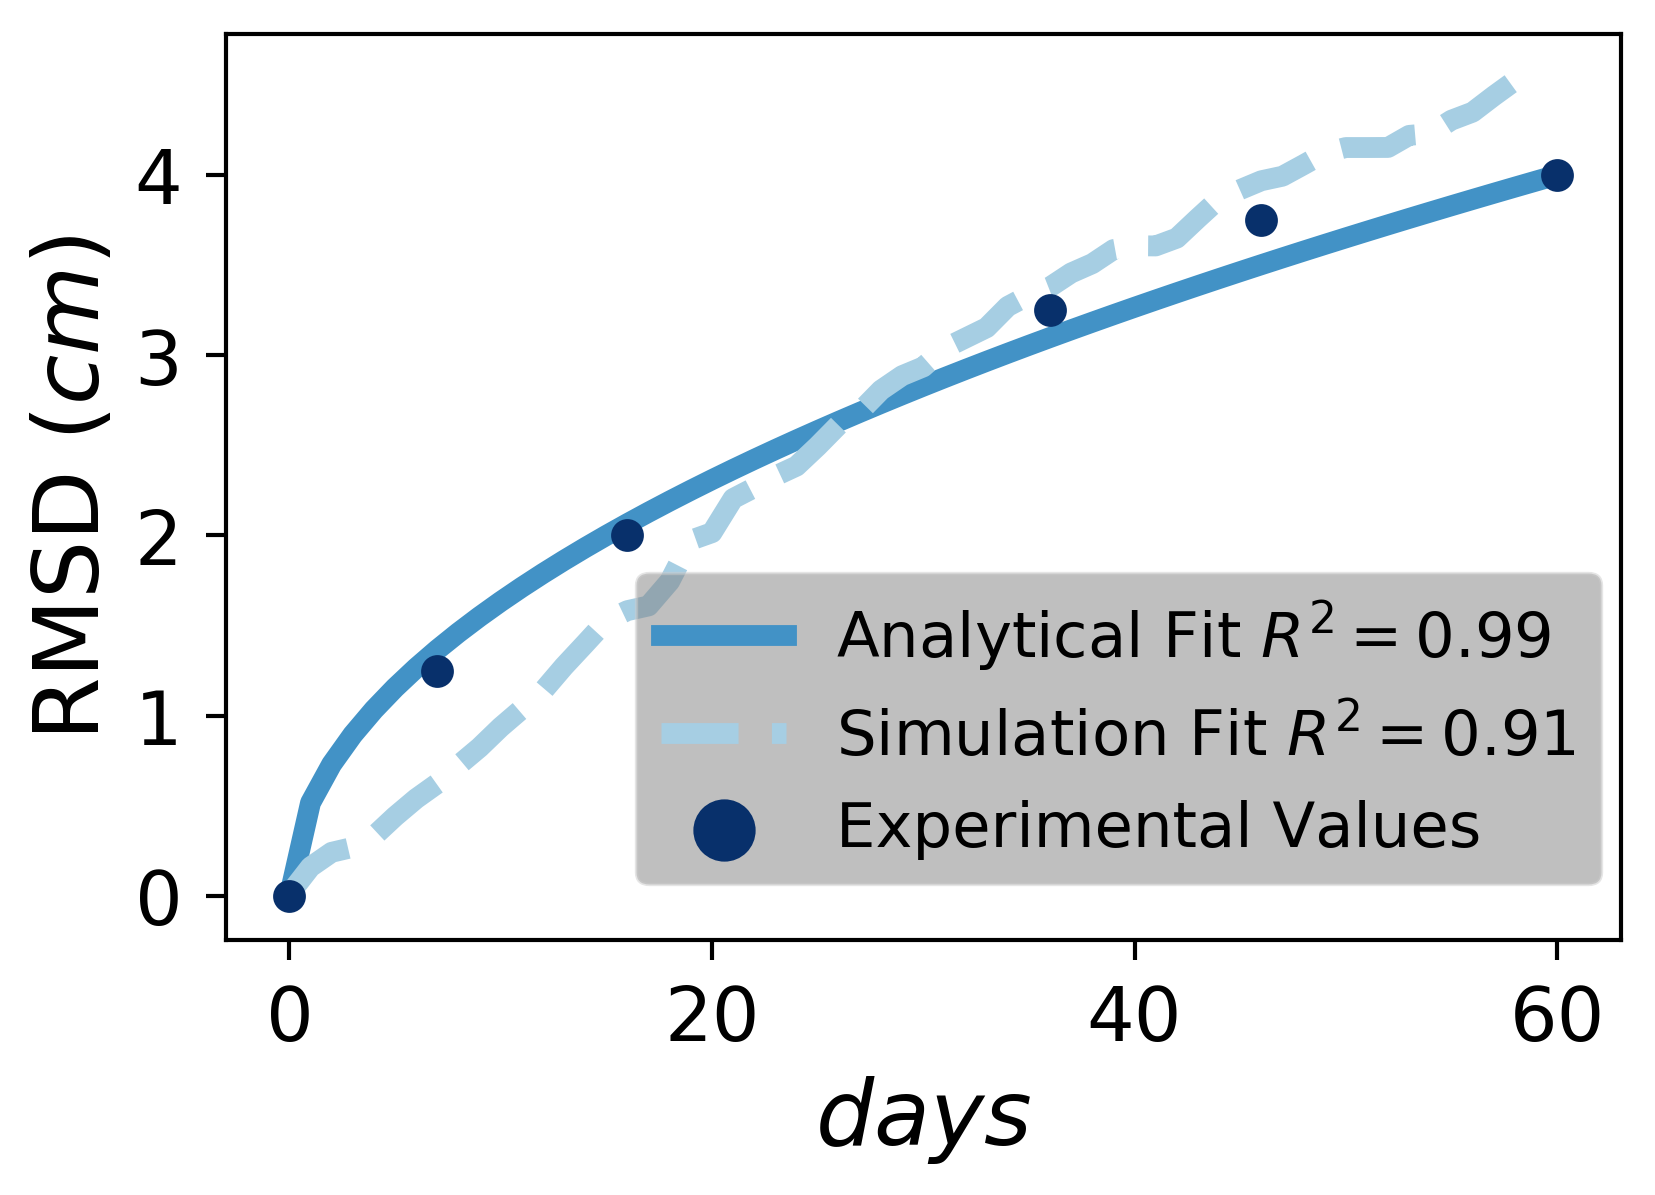
\includegraphics[width=1.0\linewidth]{fig2.png}
\caption{Comparison of model predicted RMSD (cm) (y-axis) and experimentally observed radius, for analytical $R^{2}= 0.99$ and simulation $R^{2}= 0.91$ mycelial growth over 0 to 60 days (x-axis).}
\end{figure}

\begin{figure}[h]
\centering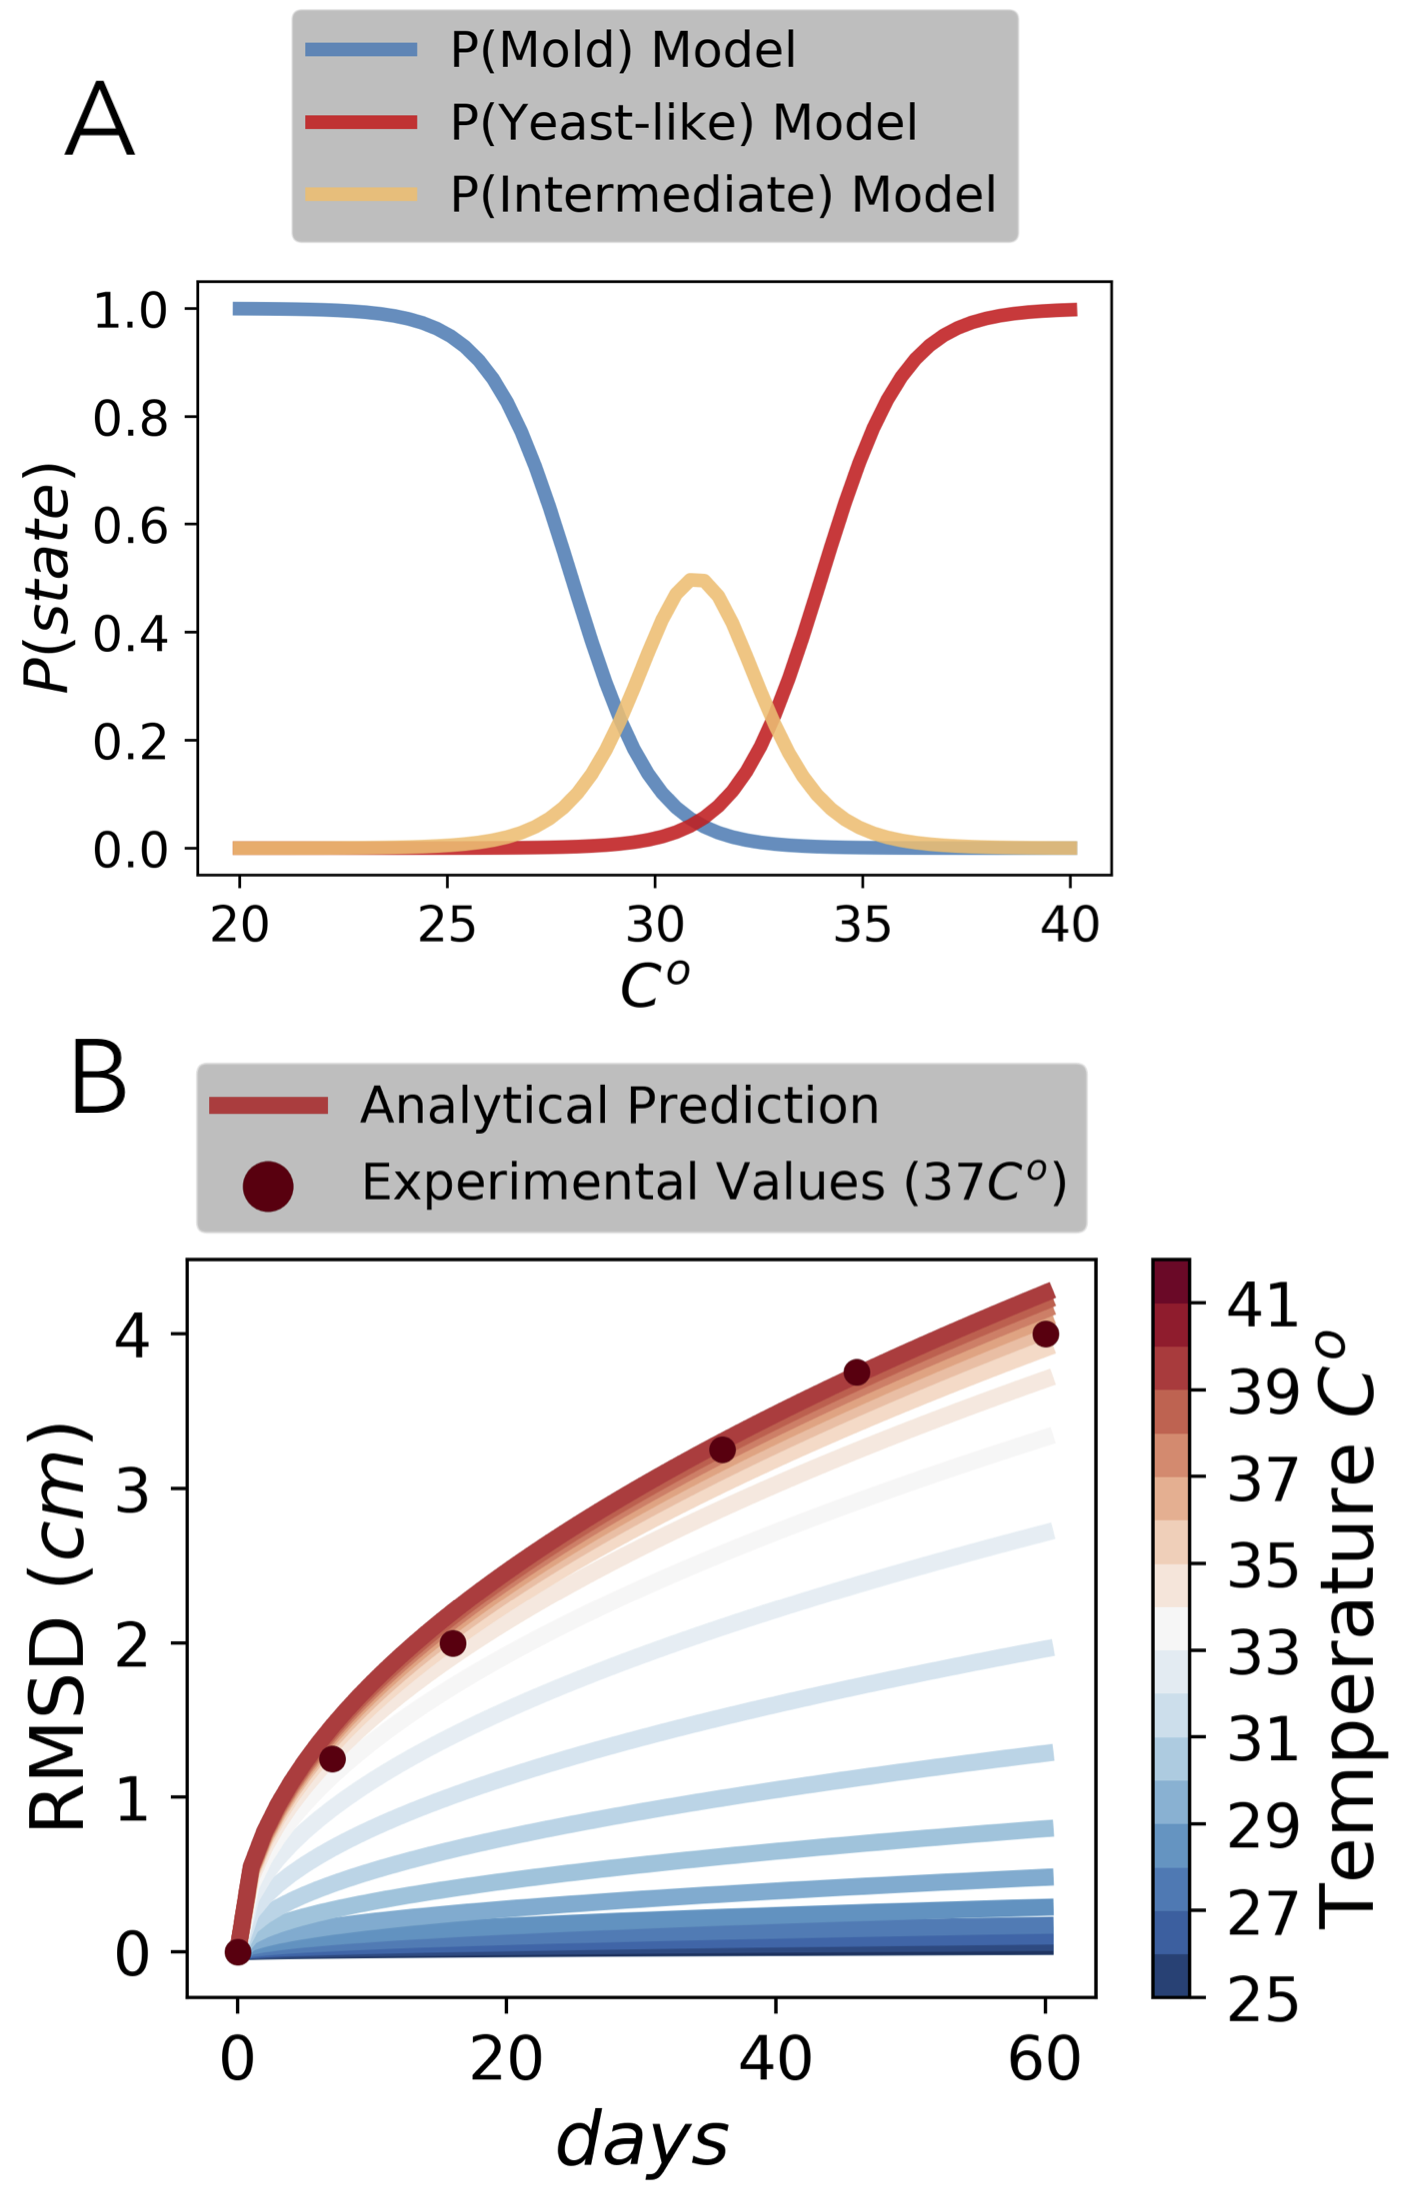
\includegraphics[width=.80\linewidth]{fig3.png}
\caption{ Two-state model predictions of \textit{B. dermatitidis} morphology proportion over temperature (A). Analytical solution of \textit{B. dermatitidis} growth as yeast-like morphology (y-axis) from 0 to 60 days (x-axis) over different temperatures (B).}
\end{figure}

\end{document}